
\section{Model\label{sec:Model}}

This section presents a Schumpeterian model based on \citeauthor{abramsPatentValueCitations2013},
featuring growth through creative destruction by entrants, as well
as the possibility for incumbent monopolist of researching a defensive
technology that increases research costs for entrants. I first present
a single-sector model to clarify the mechanism at play within each
sector in the economy and study the properties of a constant-growth
equilibrium analytically. I derive sufficient conditions under which
markup increases lower R\&D productivity, and show that this occur
only if the distribution of inventors shifts in favor of incumbent
firms carrying out defensive innovation.\footnote{In the empirical analysis, I used the HHI as a measure of concentration
and market power. Appendix \ref{app:Using-the-Lerner} shows that
the Lerner Index from NBER-CES, a standard measure of markups, is
strongly correlated with the HHI in my sample, justifying the reduced-form
mapping I adopt in this section.} I also show that in this model, when the supply of inventors is rigid,
inventors' productivity is unaffected by markup changes. Then, I move
to consider a two-sector model, where each sector is identical to
the single-sector model, and the supply of inventors is perfectly
rigid, which shuts down within-sector misallocation occurring independently
of inventors' movements across sectors. I show that increasing markups
in one of the two sectors of the economy lead to a misallocation of
R\&D resources towards defensive innovation in the less competitive
sector. Finally, I study the optimal allocation of R\&D subsidies
needed to achieve maximum growth in a calibration of the two-sector
model that matches moments of the R\&D distribution in 1997, the starting
year for my empirical analysis.

All omitted proofs are reported in Appendix \ref{app: Omitted-Proofs}.

\subsection{Single-sector Model}

\subsubsection{Preferences and production\label{subsec:Preferences-and-production}}

Consider the following continuous time economy with a single final
good. There is a representative household with King-Plosser-Rebelo
preferences over consumption and R\&D labor: 
\begin{equation}
\mathbb{E}_{t}\int_{t}^{\infty}\exp\left(-\rho\left(s-t\right)\right)\left(\ln C_{s}-\frac{\chi\left(L_{s}^{RD}\right)^{1+\frac{1}{\phi}}}{1+\frac{1}{\phi}}\right)\mathrm{d}s,\label{eq:Utility}
\end{equation}
where $\phi$ is the Frisch labor supply. In addition, the representative
household inelastically supplies $L$ units of production labor.\footnote{While this assumption is not necessary for the results to hold, it
simplifies the analysis considerably. In the following section, I
will consider both production and research labor as given by a fixed
endowment in the constant growth equilibrium of the economy. In that
case, the assumption is equivalent to assuming that both labor endowments
grow at a constant rate.} The representative household owns a differentiated portfolio of all
the firms in the economy, with rate of return $r_{t}$, and receives
a wages $w,w^{RD},$ for each unit of production and research labor,
respectively. I assume that the economy is closed and that the final
good is only used for consumption, $C_{t}=Y_{t}$. The above utility
function yields the Euler equation:
\[
\frac{\dot{C_{t}}}{C_{t}}=r_{t}-\rho,
\]
as well as a R\&D labor supply:
\[
L_{t}^{RD}=\left(\frac{w_{t}^{RD}}{\chi C_{t}}\right)^{\phi}.
\]

The consumption good in the economy in each instant is a Cobb-Douglas
aggregate of a measure-one continuum of products:
\begin{equation}
\ln Y_{t}=\int_{0}^{1}\ln y_{t}(i)\mathrm{d}i\label{eq:Y}
\end{equation}
The consumption good in the economy is taken as the numeraire. The
market for each product $y_{t}(i)$ consists of an incumbent and a
fringe of competitors. In what follows, I focus on a single market,
dropping the argument $i$. Each agent $j$ in the sector has the
linear production technology:
\[
y_{j,t}=c_{j,t}l_{j,t},
\]
where $c_{j,t}$ denotes the labor requirement for agent $j$ to produce
a unit of output, and $l_{j,t}$ denotes the production labor employed
by the firm. The incumbent and competitors produce undifferentiated
goods, and differ in their labor requirement. Competitors have labor
requirement, $c_{e,t}=c_{t}$, while the incumbent faces a lower unit
labor requirement $c_{I,t}=\frac{c_{t}}{\phi}$, with $\phi>1$. The
incumbent maximizes profits by choosing a price $p_{t}$ for her product.
Profit maximization gives an optimum limit price $p_{t}=w_{t}c_{t}$,
which leads her to capture the entire market realizing profits:
\[
\Pi_{t}=\left(c_{e,t}-c_{I,t}\right)w_{t}y_{t}=\left(\frac{\phi-1}{\phi}\right)c_{t}w_{t}y_{t}.
\]
Therefore, the incumbent acts as a monopolist, charging a markup $\phi>1$
on its marginal cost. By the Cobb-Douglas assumption on the final
good, the demand facing each product line is:
\[
y_{t}=\frac{Y_{t}}{p_{t}}=\frac{Y_{t}}{w_{t}c_{t}}.
\]
Therefore, equilibrium normalized profits read:
\[
\frac{\Pi_{t}}{Y_{t}}\equiv\pi=\left(\frac{\phi-1}{\phi}\right).
\]


\subsubsection{Innovation}

Both incumbents and entrants can conduct innovation activity that,
if successful, reduces their unit costs to

\[
c_{I,t+\Delta_{t}}=\frac{c_{e,t}}{\left(1+\eta\right)\phi},\quad\eta>1
\]
Here, $\eta$ parametrizes the percentage increase in productivity
for the innovating firm, relative to the technology previously operated
by the incumbent. I assume that there are spillovers from realized
innovations as follows. Whenever either the incumbent or an entrant
realize an innovation, all other firms gain access to a technology
with unit costs
\[
c_{e,t+\Delta_{t}}=\frac{c_{e,t}}{\left(1+\eta\right)}.
\]
These assumptions imply that, if entrants realize an innovation, they
outcompete previous incumbents, and become the new monopolists. Displaced
incumbents join the pool of entrants and from instant $t+\Delta t$
onwards operate the technology $c_{e,t+\Delta_{t}}$. This amounts
to assuming that the incumbent's technology becomes obsolete after
displacement.\footnote{An alternative interpretation of this assumption is that incumbents
are forced to scrap the assets needed to operate the innovative technology
upon destruction, so that the technology is no longer available to
them from the following instant onwards. } Technically, this innovation structure allows to avoid keeping track
of the number of realized innovations. Indeed, in each product market
the relative productivity of incumbents relative to entrants is fixed
at $\phi$, making it possible to formulate the choice of innovation
as a recursive problem.

Incumbents' and entrants' innovation differ in two respects. First,
successful incumbents' R\&D produces a \emph{patent wall }of size
$\omega>1$, which decreases the success probability of entrants'
innovations. Second, successful entrants' R\&D results in an implemented
innovation with certainty, while incumbents adopt new technologies
with probability, $\lambda\in[0,1].$ This parameter can be interpreted
in two ways. The first interpretation is that $\lambda$ captures
the probability that the newly discovered technology is compatible
with the incumbents' current production techniques. The second interpretation
is related to the radical nature of incumbents' innovations. A low
value for $\lambda$ reduces the expected productivity improvement
from an innovation by the incumbent. In other words, the lower $\lambda,$
the more incremental are incumbents' innovations. Under these assumptions,
incumbents \emph{always} obtain a patent wall, but they only implement
their innovations with probability $\lambda$.\footnote{This specification connects to the empirical evidence in \citet{argentePatentsProductsProduct2020a},
who show that large incumbent firms tend to produce a large amount
of patents, but implement a small number of product innovations.}

Following \citet{acemogluIntellectualPropertyRights2012}, I assume
that innovation investments consist in the choice of an arrival rate
of new discoveries, $x_{I}$, and that R\&D costs are increasing and
convex in this arrival rate. In particular, I specify incumbents'
R\&D costs as:
\[
C\left(x_{I};w^{RD}\right)=\alpha_{I}\frac{x_{I}^{\gamma}}{\gamma}w^{RD},\ \gamma>1,
\]
where the term, $\alpha_{I}\frac{x_{I}^{\gamma}}{\gamma}$, indicates
the amount of inventors that the incumbent needs to obtain innovations
with a flow probability, $x_{I},$and $w^{RD}$ is the wage paid to
inventors. For simplicity, I assume that incumbents can only have
one available innovation at a time. That is, incumbents can only erect
\emph{one} patent wall of size $\omega>1$, and cannot invest in further
innovation until this wall is destroyed at a rate, $\delta$, which
captures the rate of patent expiration.

Given these assumptions incumbents' values at any given instant are
just a function of the state of the patent wall in the product market
they operate, $\Omega\in\left\{ 1,\omega\right\} .$ Given the recursive
nature of the problem, I drop time indexes in what follows. Incumbents'
value functions read:
\begin{align}
rV(1)-\dot{V}(1) & =\max_{x_{I}}\left\{ \left(\frac{\phi-1}{\phi}\right)Y-\alpha_{I}\frac{x_{I}^{\gamma}}{\gamma}w^{RD}+x_{I}\left(V(\omega)-V(1)\right)-x_{e,1}V(1)\right\} ,\label{eq:v_1}\\
rV(\omega)-\dot{V}(\omega) & =\left(\frac{\phi-1}{\phi}\right)Y+\delta\left(V(1)-V(\omega)\right)-x_{e,\omega}V(\omega),\label{eq:v_om}
\end{align}
where $x_{e,1}$, $x_{e,\omega}$ denote entrants' innovation intensities,
$r$ is the interest rate in the economy to be determined in equilibrium,
and $\delta$ the rate of patent expiration. The first line displays
the flow value to incumbents that operate in a market not protected
by a patent wall. There, incumbents realize instantaneous profits,
$\left(\frac{\phi-1}{\phi}\right)Y$, and choose their innovation
intensity, $x_{I}$, taking the researchers' wage, $w^{RD}$, as well
as the entrants' innovation intensity $x_{e,1}$, as given. If entrants
are successful at rate $x_{e,1}$, incumbents are destroyed. If incumbents'
innovation is successful at rate, $x_{I}$, they obtain the patent
wall $\omega$, which grants them the protected value, $V(\omega)$.
When a patent wall is in place, incumbents realize the same flow profits
as in the unprotected state, since economy-wide spillovers imply that
incumbents are unable to reap profits from implemented innovations.
However, incumbents face a different entrants' innovation intensity,
$x_{e,\omega}$, which is lower than $x_{e,1}$ due to the patent
wall in place, as I will show below. Finally, incumbents in state
$\omega$ face a flow probability $\delta$ that the patent wall is
exogenously destroyed, in which case they transition back to the unprotected
state. Under these assumptions, the optimal incumbent's R\&D decision
is given by:
\begin{equation}
x_{I}=\bm{1}\left\{ V(\omega)-V(1)>0\right\} \left(\frac{V(\omega)-V(1)}{\alpha_{I}w^{RD}}\right)^{\frac{1}{\gamma-1}}.\label{eq:RD_I}
\end{equation}

Following \citeauthor{abramsPatentValueCitations2013}, I assume that
each market has a mass of atomistic entrants, indexed by $j$, who
face innovation costs that feature congestion externalities:
\[
C\left(x_{e,\Omega,j};w^{RD}\right)=\zeta\Omega x_{e,\Omega,j}x_{e,\Omega}w^{RD}.
\]
In this specification, $\zeta$ parametrizes the inventor requirement
to obtain a unit aggregate entrants' innovation rate when the market
is not protected by patent walls, $\Omega=1$. Individuals costs are
linear in the total entrants' research intensity in the product market,
$x_{e,\Omega}\equiv\int_{\mathcal{J}}x_{e,\Omega,j}\mathrm{d}j.$
In other terms, individual entry costs increase with the aggregate
entry rate. I assume that successful entrants obtain a new unprotected
technology, regardless of the state of the market that they target,
capturing the fact that entrants do not obtain the patents deposited
by the previous incumbents, instead implementing entirely new production
techniques. 

Under the above assumptions, the free entry condition for entrants
targeting a market with patent wall $\Omega$ reads:

\[
\max_{x_{e,\Omega,i}}\left\{ x_{e,\Omega,i}V(1)-\zeta\Omega x_{e,\Omega,i}x_{e,\Omega}w^{RD}\right\} .
\]
This condition pins down the entry rate for each product market with
patent wall $\Omega$ as:
\begin{equation}
x_{e,\Omega}=\frac{V(1)}{\zeta\Omega w^{RD}},\quad\Omega\in\{1,\omega\}.\label{eq:RD_e}
\end{equation}
This expression clarifies the effect of defensive innovation in this
model. The size of the patent wall $\omega$ represents the factor
decrease in the entry rate when a defensive innovation is successful. 

\subsubsection{Equilibrium with Constant Growth}

The laws of motion of product markets across protected and unprotected
states is given by:
\begin{align}
\dot{\mu}_{1} & =-\left(x_{I}+x_{e,1}\right)\mu_{1}+\delta\mu_{\omega}+x_{e,\omega}\mu_{e,\omega}+x_{e,1}\mu_{e,1},\label{eq: dist1-1}\\
\dot{\mu}_{\omega} & =-\left(x_{e,\omega}+\delta\right)\mu_{\omega}+x_{I}\mu_{1},\label{eq: dist2-1}
\end{align}
where $\mu_{e,\omega}$ and $\mu_{e,1}$ denote the mass of entrants
targeting protected and unprotected markets, respectively. Equation
(\ref{eq: dist1-1}) states that the mass of unprotected products
decreases when incumbents successfully develop an innovation at flow
probability, $x_{I},$ or entrants displace existing incumbents at
rate, $x_{e,1}$. Products instead become unprotected if existing
patent walls depreciate, or successful entrants become new monopolists.
Conversely, Equation (\ref{eq: dist1-2}) shows that protected markets
loose mass whenever entrants displace existing protected incumbents
or defensive patents depreciate, and gain mass when incumbents in
unprotected markets develop defensive innovations. 

The mass of entrants in the two types of product markets is determined
in equilibrium following the laws of motion:

\begin{align}
\dot{\mu}_{e,1} & =-\left(x_{e,1}+x_{I}\right)\mu_{e,1}+x_{e,1}\mu_{1}+\delta\mu_{e,\omega},\label{eq: dist3-1}\\
\dot{\mu}_{e,\omega} & =-\left(x_{e,\omega}+\delta\right)\mu_{e,\omega}+x_{e,\omega}\mu_{\omega}+x_{I}\mu_{e,1}.\label{eq: dist4-1}
\end{align}
Here, the first line states that the pool of entrants in unprotected
markets looses mass if entrants successfully develop innovations at
rate, $x_{e,1},$ or incumbents make markets protected at rate, $x_{I}.$
The pool of entrants in markets with $\Omega=1$ instead grows when
incumbents get displaced by successful entrants, and rejoin the ranks
of outsiders, or previously protected markets loose their defensive
walls. Equation (\ref{eq: dist4-1}) is obtained analogously. Given
research intensities, clearing in the labor markets for production
and research labor require:
\begin{align}
L & =\int_{0}^{1}l(i)\mathrm{d}i,\label{eq: Lprod}\\
L^{RD} & =\zeta\left(\omega x_{e,\omega}\mu_{e,\omega}+x_{e,1}\mu_{e,1}\right)+\alpha_{I}\frac{x_{I}^{\gamma}}{\gamma}\mu_{1}.\label{eq: LRD}
\end{align}

A constant growth equilibrium of this economy is defined as follows.
\begin{defn}[Constant Growth Equilibrium]
 A constant growth equilibrium is a sequence of values $\left\{ V_{t}(1),V_{t}(\omega)\right\} ,$
production workers' and inventors' wage sequences $\left\{ w_{t}^{RD},w_{t}\right\} $,
and incumbents' and entrants' R\&D decisions $\left\{ x_{I,t},x_{e,1,t},x_{e,\omega,t}\right\} $
such that, given an endowment of production labor, $L$, $L^{RD}$:
(i) incumbents maximize values (\ref{eq:v_1}) and (\ref{eq:v_om}),
taking entrants R\&D decisions as given, (ii) entrants' R\&D decisions
satisfy (\ref{eq:RD_I}) and (\ref{eq:RD_e}) taking $V_{t}(1)$ as
given, (iii) the distribution of incumbents and entrants across protected
and unprotected markets is constant, $\dot{\mu}_{1}=\dot{\mu}_{\omega}=\dot{\mu}_{e,1}=\dot{\mu}_{e,\omega}=0$
in Equations (\ref{eq: dist1-1})-(\ref{eq: dist4-1}), (iv) values
in each instant are determined by (\ref{eq:v_1}) and (\ref{eq:v_om}),
(v) consumers maximize utility (\ref{eq:Utility}) choosing consumption
and R\&D labor optimally, (vi) labor markets clear according to (\ref{eq: Lprod})
and (\ref{eq: LRD}), (vii) product markets clear, $C_{t}=Y_{t}$,
and (vi) aggregate output (\ref{eq:Y}) grows at the constant rate,
$g\equiv\dot{Y}_{t}/Y_{t}.$
\end{defn}
The following proposition summarizes the properties of the constant
growth equilibrium.
\begin{prop}[Existence and Uniqueness of the Constant Growth Equilibrium]
 \label{prop:CGE}For any endowments of production labor, $L$, there
exists a unique constant growth equilibrium. Denoting optimal incumbents'
and entrants' choices as $x_{I}^{\star},x_{e,\omega}^{\star},x_{e,1}^{\star},$
and the masses of incumbents and entrants across states as $\mu_{1}^{\star},\mu_{\omega}^{\star},\mu_{e,1}^{\star},\mu_{e,\omega}^{\star}$,
the constant growth rate of the economy is given by:
\[
g=\eta\left[x_{e,\omega}^{\star}\mu_{e,\omega}^{\star}+x_{e,1}^{\star}\mu_{e,1}^{\star}+\lambda x_{I}^{\star}\mu_{1}^{\star}\right],
\]
and inventors' productivity is given by:
\[
\frac{g}{L^{RD}}=\eta\frac{x_{e,\omega}^{\star}\mu_{e,\omega}^{\star}+x_{e,1}^{\star}\mu_{e,1}^{\star}+\lambda x_{I}^{\star}\mu_{1}^{\star}}{\zeta\left(\omega x_{e,\omega}^{\star}\mu_{e,\omega}^{\star}+x_{e,1}^{\star}\mu_{e,1}^{\star}\right)+\alpha_{I}\frac{\left(x_{I}^{\star}\right)^{\gamma}}{\gamma}\mu_{1}^{\star}}.
\]
\end{prop}
%
The expression for inventors' productivity can be used to obtain a
first intuition of the mechanism through which higher markups lead
to decreased productivity in this model. First, note that a unit of
total entrants' research intensity in either protected and unprotected
markets produces the same growth. Indeed, by the expression for growth,
it is clear that a unit increase in either $x_{e,\omega}^{\star}\mu_{e,\omega}^{\star}$
or $x_{e,1}^{\star}\mu_{e,1}^{\star}$ gives a growth of $\eta$.
However, the unit labor requirement of research intensity in protected
markets is larger than in unprotected markets as a result of defensive
patents. This is evident from the first term at the denominator, that
shows that a unit of total research in protected markets requires
$\zeta\omega$ inventors, compared with just $\zeta$ in unprotected
markets. These facts immediately imply that any force that pushes
entrants towards protected markets will lower their inventor productivity.
One such force is an increase in incumbents' research intensity that
outstrips entrants', which acts to increase $\mu_{e,\omega},$ the
mass of entrants active in protected markets. As I show formally below,
an increase in the markup raises the value of monopolistic positions,
which pushes up both incumbents' and entrants' research intensities,
$x_{I},x_{e,\omega}.$ This results in an increase in $\mu_{e,\omega}$
only if incumbents' R\&D intensity is more elastic than entrants'. 

The following proposition states the main result in this section,
showing that higher markups unambiguously increase research efforts
by incumbents and entrants, and the share of R\&D labor accruing to
incumbents. The proposition also states the main condition for this
result to lead to a fall in overall inventors' productivity in terms
of sufficient statistics. In particular, the incumbents' R\&D elasticity
to markups must be larger than entrants'. This condition is satisfied
in the data, as the estimates in Table \ref{tab: RegStats}, which
show that incumbents increase their share of inventors following increases
in markups. 
\begin{prop}[Effects of Markup Increases on Innovation]
\label{prop: partialEq}Suppose that defensive research is effective,
$\omega>1$. The constant growth equilibrium features positive incumbents'
research, $x_{I}^{\star}>0$, and markup increases raise both incumbents'
and entrants' research effort:
\[
\frac{\partial x_{I}^{\star}}{\partial\phi}>0,\ \frac{\partial x_{e,\omega}^{\star}}{\partial\phi}>0\ \frac{\partial x_{e,1}^{\star}}{\partial\phi}>0,
\]
and the share of R\&D labor employed by incumbents increases with
markup:
\[
\frac{\partial\frac{L_{I}}{L^{RD}}}{\partial\phi}=\frac{\partial\left(\nicefrac{\alpha_{I}\frac{x_{I}^{\gamma}}{\gamma}\mu_{1}}{L^{RD}}\right)}{\partial\phi}>0.
\]
Moreover, if $\lambda=0,$ inventor supply is not fully inelastic,
and the model parameters are such that equilibrium incumbents' research
effort is more elastic than entrants', 
\[
\frac{\partial x_{I}^{\star}}{\partial\phi}\frac{\phi}{x_{I}^{\star}}>\frac{\partial x_{e,\omega}^{\star}}{\partial\phi}\frac{\phi}{x_{e,\omega}^{\star}},
\]
it further holds:
\[
\frac{\partial\left(\nicefrac{g}{L^{RD}}\right)}{\partial\phi}<0.
\]
That is, an increase in the markup, $\phi$, lowers equilibrium inventors'
productivity. 
\end{prop}
The intuition behind this proposition is that increases in the markup
raise the value of monopolistic positions, thus raising both entrants'
and incumbents' research effort. In addition, this leads to an overall
increase in inventors employed by incumbents. Importantly, this holds
only if defensive R\&D is effective, showing the importance of this
channel to reproduce the empirical findings in Table \ref{tab: RegStats}.
However, this finding is not sufficient to generate a fall in inventors'
productivity. This is because the overall change in inventors' productivity
can be decomposed as:
\begin{align*}
\mathrm{d}\left(\frac{g}{L^{RD}}\right) & =\mathrm{d}\left(\frac{L_{e}}{L^{RD}}P_{e}\right)+\mathrm{d}\left(\frac{L_{I}}{L^{RD}}P_{I}\right),
\end{align*}
where $P_{e}$, $P_{I}$ denote entrants' and incumbents' productivity,
respectively. As long as incumbents' productivity is lower than entrants,
a reallocation of inventors towards dominant firm leads to a decrease
in inventors productivity. However, this effect can in principle be
offset by an increase in entrants' productivity. The sufficient conditions
in Proposition \ref{prop: partialEq} ensure that this is not the
case.\footnote{Corollary \ref{cor: parameters} in the Appendix provides parametric
sufficient conditions for the case with quadratic costs, $\gamma=2$,
which is analytically tractable.} In particular, if incumbents' research effort is more elastic than
entrants', an increase in markups reduces the overall share of unprotected
markets, making entry overall more difficult, and reducing entrants'
productivity as well. This reasoning also clarifies why the condition
is sufficient. Indeed, a fall in inventors' productivity occurs as
long as the increase in creative-destruction growth by entrants is
not high enough relative to the increase in defensive innovation by
entrants. As noted above, this condition is satisfied in the data,
and always appear to be in numerical simulations, regardless of specific
assumptions on parameter values. In particular, the assumption $\lambda=0$
is not necessary to generate the result, but I make to obtain clear
analytical results in the proof to this Proposition. 

It is important to stress that the decline in productivity requires
a strictly positive elasticity of inventors' supply. As I show in
Lemma \ref{lem:Labor Demand} in the Appendix, \emph{aggregate} inventor
labor demand is increasing in markups. As a result, when inventors'
supply is fully rigid, wage effects need to fully offset the increase
in labor demand, and by the uniqueness of the CGE, it the allocation
of inventors across incumbents and entrants is fixed. Indeed, aggregate
labor demand is uniquely pinned down by research intensities through
the stationary distribution. 

Figure \ref{fig:OneSecCS} provides a graphical illustration of the
comparative statics for an increase in markup in a calibration of
the one-sector model, which follows the strategy described in detail
in the following Section.\footnote{The parameters of the calibration are chosen to match moments of the
R\&D expenditure distribution as in Section \ref{subsec:Two-sectors},
and the complete set of parameters is reported in Appendix. } An increase in the markup raises profits, thereby increasing the
value of dominant positions, and propelling both incumbents' and entrants'
research. Importantly, the incumbents' inventor demand is more elastic
to increased profits, which raises the overall proportion of researchers
employed in defensive projects. Although overall growth increases
as a result of higher aggregate R\&D, the productivity of inventors
fall, as they get increasingly allocated to incumbents. Two observations
are in order. First, with a fixed supply of inventors, equilibrium
allocations do not change with increased profits, leaving R\&D productivity
unaffected. Second, in the absence of defensive innovation, the increase
in profits would just result in increased entry and growth, leaving
productivity constant.\footnote{In the absence of defensive innovation, the whole mass of firms operates
in unprotected markets and there is no incumbent research. From the
expression for growth in Proposition \ref{prop: partialEq} inventor
productivity is constant at $\nicefrac{\eta}{\zeta}.$}

\begin{figure}[th]
\begin{centering}
\caption{Comparative Statics for Changes in the Markup in the Single-Sector
Model \label{fig:OneSecCS}}
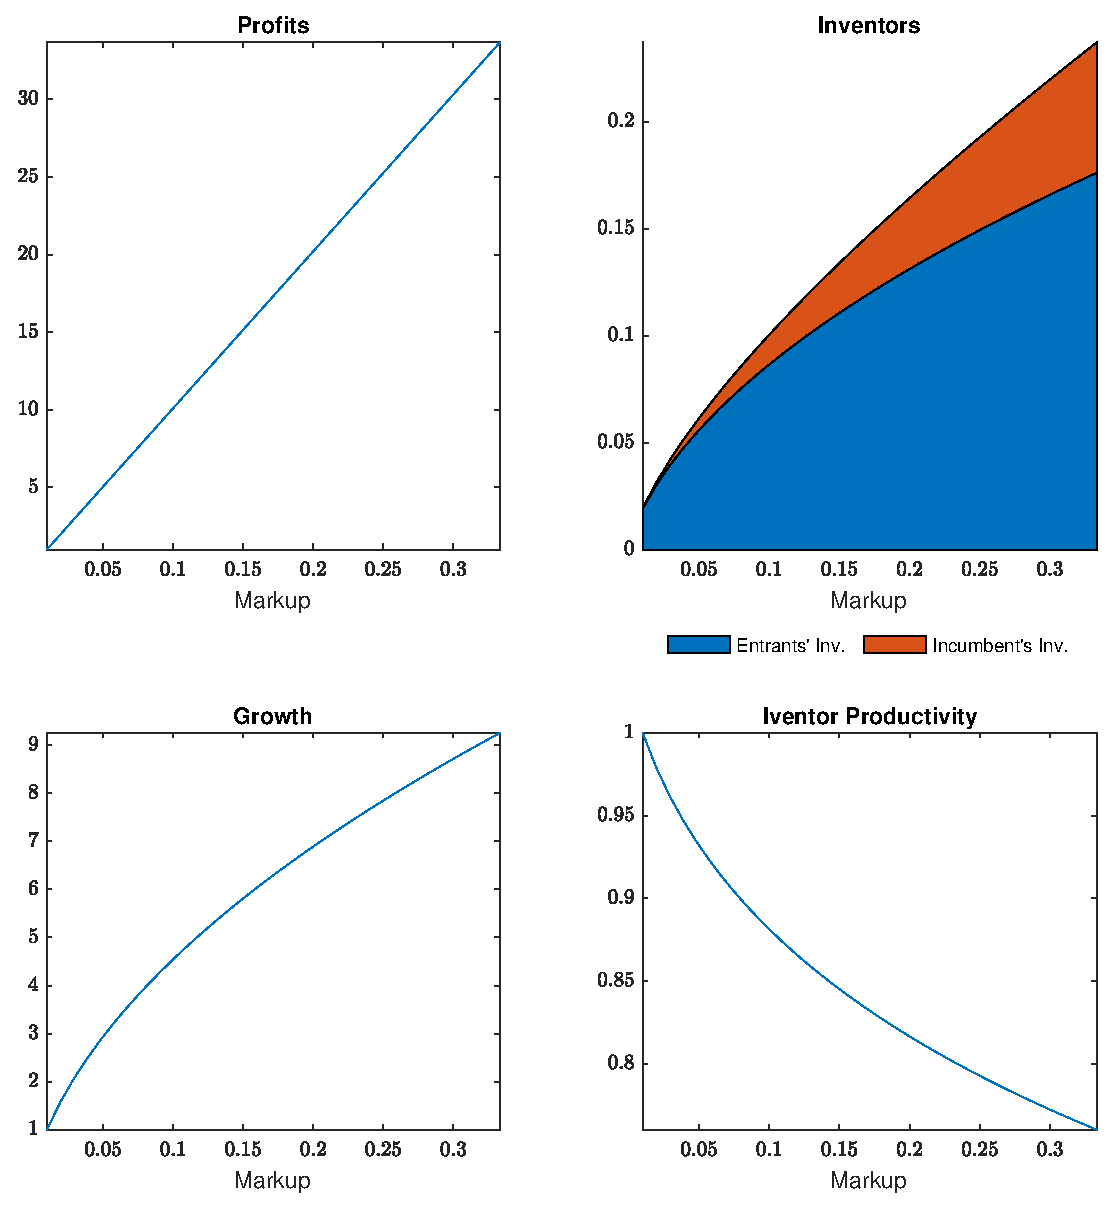
\includegraphics[width=1\textwidth]{graphs/Single_sector}
\par\end{centering}
\raggedright{}{\small{}Note: This figure reports the comparative statics
for normalized profits, inventors, growth and inventor productivity
in the single-sector model. All variables are expressed in units relative
to the equilibrium with $\phi=1.08.$ The calibration follows the
same strategy as in Section \ref{subsec:Calibration}, assuming that
the economy is only composed by a single sector. I set the elasticity
of inventors' supply at $\varphi=1$. }{\small\par}
\end{figure}
\FloatBarrier

\subsection{Calibration and Policy\label{subsec:Two-sectors}}

In this section, I calibrate a two-sector extension of the model presented
in the previous Section, with two main objectives. First, I want to
analyze misallocation \emph{across }sectors, and show that, under
a realistic calibration, this extension can qualitatively reproduce
the main findings of the empirical analysis. I focus on the benchmark
with\emph{ fixed} inventor supply where, by the results in the previous
section, markups have no effect on inventors' productivity within
sectors. This choice excludes that my findings are driven by within-sector
misallocation alone. Second, I wish to study the distribution of R\&D
subsidies across firms that maximizes aggregate growth. The policy
analysis reveals that a planner interested in maximizing growth chooses
to subsidize entry in less competitive sectors, rather than reallocating
inventors back to more competitive sectors. This result arises for
two reasons. First, while misallocation arises only as a result of
flows across sectors, it acts through misallocation within the sector
that becomes more concentrated, where incumbents' defensive research
increases more than entrants' productive R\&D. Second, the outflow
of inventors reduces defensive innovation more competitive sectors.
As a result, reallocating inventors back to competitive sectors would
then come at the cost of inventor productivity in these sectors, while
tackling the misallocation within concentrated sectors only indirectly.

\subsubsection{Model description}

The consumption good in the economy is given by the Cobb Douglas aggregate:
\[
\ln Y_{t}=\beta_{1}\ln Y_{1,t}+\beta_{2}\ln Y_{2,t},\quad\beta_{1}+\beta_{2}=1
\]
where $Y_{1,t}$, $Y_{2,t}$ are produced as in Section \ref{subsec:Preferences-and-production},
and the markup parameter, $\phi$, is allowed to vary across the two
sectors.

The household side of the economy is unchanged relative to the one-sector
model. In this section, however, the supply of inventors is assumed
to be fully rigid and given by $L^{RD}=100.$ This assumption is motivated
by two considerations. First, a fixed inventor supply captures an
aggregate scarcity of inventors, allowing me to focus exclusively
on their allocation across sectors. Second, as discussed above, in
this benchmark markup changes have no effect on misallocation if inventors
are not allowed to move across sectors. Therefore, the results below
isolate the effect of inventors' transitions across sectors on misallocation.

Given the presence of two markets, labor market clearing for production
workers and inventors is now given by:
\begin{align}
L & =\sum_{i=1}^{2}\int_{0}^{1}l_{i,j,t}\left(w^{RD}\right)\mathrm{d}j,\label{eq: Lprod-1}\\
L^{RD} & =\sum_{i=1}^{2}L_{i,t}^{RD}\left(w^{RD}\right),\label{eq: LRD-1}
\end{align}
where the subscript $i$ denotes sectors and $j$ the product markets
in each sector. I define a constant growth equilibrium as in the previous
section. Given the Cobb-Douglas assumption on the final good, growth
is now given by:
\[
\Delta\ln Y_{t}=\sum_{i=1}\beta_{i}g_{i},
\]
where $g_{i}$ denotes the sector-specific output growth obtained
as in Proposition \ref{prop: partialEq}. Appendix \ref{app: twoSec}
reports the derivations for the two-sector model and a complete description
of the equations characterizing the equilibrium.

\subsubsection{Calibration\label{subsec:Calibration}}

I calibrate my model in order to match features of the R\&D distribution
and concentration around 1997, the starting year for my analysis.
The aim of my calibration is to provide a qualitative description
of the features of the model under realistic parameter choices. For
this reason, I do not attempt to match the fall in growth implied
by the model within or across sectors. As I will show below, my calibration
implies a fall in inventors' productivity of about 2\% over the period
1997-2012, about half of the lower bound implied by my empirical estimates.
The calibration is therefore very conservative relative to my empirical
estimates, which provides a useful benchmark to establish a lower
bound of the effects of switching to an optimal R\&D subsidy policy
in the following section. 

Table \ref{tab: intPar} displays my choices for parameters calibrated
externally. I set the discount rate to $4\%$, which, together with
a 3\% growth for my sample in 1997, implies a value for the real interest
rate of 7\%, in line with the long-run average before 1997. I obtain
a value for $\beta$, the share of value added of each sector, from
estimates of the Lerner Index in manufacturing that I obtain from
the NBER-CES as described in Appendix \ref{app:Using-the-Lerner}.
According to these estimates, about half of the sectors (weighted
by sales) for which I have these data saw an increase in the Lerner
Index over the period. This suggests $\beta_{1}=\beta_{2}=0.5.$ Since
I only have the Lerner Index for about half of the sectors, I rely
on the extensive literature estimating markups to set a value of $\phi=1.08$.
In particular, I follow \citet{akcigitWhatHappenedBusiness2019a},
who calibrate the same parameter using the midpoint of estimates provided
in \citet{deloeckerRiseMarketPower2020} and \citet{eggertssonKaldorPikettyFacts2018}.
As standard in the literature \citep[see e.g., ][]{acemogluIntellectualPropertyRights2012},
I set the curvature of the incumbents' cost function relying on the
estimates by \citealp{kortumEquilibriumPatentRatio1993}. I choose
the lower bound of these estimates in order to minimize the asymmetry
of innovation costs between incumbents and entrants, as more convex
incumbents' costs mechanically make incumbents' research, even when
productive, less effective than entrants. The rate of patent expiration
comes directly from the legislative framework in the US, as established
by the Uruguay Round Agreements Act of 1994. Since $\lambda$ measures
how radical are incumbents' innovations relative to entrants', I set
$\lambda=0.785$, the complement of the internal patent share of 21.5\%
estimated by \citet{akcigitGrowthHeterogeneousInnovations2018}. Turning
to the value of blocking patents, parametrized by $\omega$ in my
model, I rely on estimates by \citet{czarnitzkiHowValuableAre2020}
and \citet{grimpePreemptingTechnologyCompetition2008}, who employ
merger data to obtain the effect of pre-emptive patents on the value
of acquired firms. Both their estimates imply an elasticity of firm's
values to the share of patents with pre-emptive value of more than
one. This implies that a firm with a patent portfolio composed exclusively
of defensive patents is valued on average twice as much as one with
only patents that have no pre-emptive value. This suggest a value
of $\omega=2$. As shown in the proof of Proposition \ref{prop:CGE},
my model gives an elasticity of firms' value of at most $\omega-1$,
therefore $\omega=2$ effectively caps this elasticity to $1$. I
also include R\&D subsidies, modeled as a percent subsidy on inventors'
wages,$s$, and corporate taxes applied to firms instantaneous profits,
$\tau$. I set these two parameters following the values reported
by \citet{akcigitOptimalTaxationPolicies2016}.

Table \ref{tab: intPar} describes my choices for the remaining parameters,
that govern the scale of R\&D and the growth rate in the economy.
Specifically, I set the incumbents' and entrants' R\&D cost scale,
$\alpha_{I}$ and $\zeta$, in order to match the share of inventors
employed by incumbent firms in 1997 and the R\&D business spending
as a percent of GDP, as reported by the National Science Foundation.
Intuitively, the two cost parameters jointly determine the overall
R\&D spending in the economy, while their relative value determines
the distribution of R\&D spending in equilibrium. Given the estimates
for $\alpha_{I}$ and $\zeta$, I set $\eta$ to match the growth
in output per worker for the sectors considered in my analysis in
1997, $3.03\%$. All targets are matched almost exactly.\footnote{The average percentage point deviation of moments in the model from
their empirical targets is less than $10^{-6}.$} 

\begin{sidewaystable}
\caption{Parameter Values and Sources}
\subfloat[Parameters Calibrated Externally]{\label{tab: extPar}
\centering{}%
\begin{tabular}{llll}
\toprule 
Parameter Name & Symbol & Value & Source/Target\tabularnewline
\midrule
\midrule 
Discount rate & $\rho$ & .04 & Annual real interest rate $\approx7\%$ before 1997\tabularnewline
Value Added Share & $\beta$ & .5 & Share of sectors with $\uparrow$ Lerner Index\tabularnewline
Average Sectors' Markup & $\phi$ & 1.08 & \citealp{deloeckerRiseMarketPower2020} and \citealp{eggertssonKaldorPikettyFacts2018}\tabularnewline
Innovation Cost Curvature & $\gamma$ & $1/.6$ & Lower bound of estimates in \citealp{kortumEquilibriumPatentRatio1993}\tabularnewline
Intensity of Patent Expiration & $\delta$ & .05 & Uruguay Round Agreements Act (1994)\tabularnewline
Share of Implemented Innovations & $\lambda$ & .785 & Internal patent share of 21.5\% \citep{akcigitGrowthHeterogeneousInnovations2018}\tabularnewline
Value of Blocking Patents & $\omega$ & 2 & \citealp{czarnitzkiHowValuableAre2020,grimpePreemptingTechnologyCompetition2008}\tabularnewline
R\&D subsidy  & $s_{I}=s_{e}$ & 19\% & \citealp{akcigitOptimalTaxationPolicies2016}\tabularnewline
Corporate tax rate  & $\tau$ & 23\% & \citealp{akcigitOptimalTaxationPolicies2016}\tabularnewline
\bottomrule
\end{tabular}}\\

\centering{}\subfloat[Parameters Calibrated Internally]{\label{tab: intPar}
\centering{}%
\begin{tabular}{lccc}
\toprule 
Parameter Name & Symbol & Value & Target\tabularnewline
\midrule
\midrule 
Incumbent Costs & $\alpha_{I}$ & 21.97 & Top 10\% Firms' Inventor Share, 1997: 30.3\%\tabularnewline
Entrants' Costs & $\zeta$ & 4.75 & Business R\&D Share over GDP, 1997: 1.81\%\tabularnewline
Innovation Step & $\eta$ & 0.0047 & Output per Worker Growth, 1997: 3.03\%\tabularnewline
\bottomrule
\end{tabular}}
\end{sidewaystable}


\subsubsection{Comparative Statics in General Equilibrium}

Figure \ref{fig:TwoSecAgg} displays the comparative statics for an
increase in markup in sector 2, while leaving the other sector's markup
unchanged. The graphs compares the aggregates of interest across different
constant growth equilibria, and each figure reports the markup of
sector 2 relative to sector 1 on the x-axis. 

An increase in the relative markup of sector 2 leads to a pronounced
reallocation of inventors away from sector 1. In sector 2, incoming
inventors are allocated disproportionately to incumbents, who expand
their share of researchers relative to entrants. This leads to a decrease
in overall inventor productivity of about Computing the Lerner Index
on NBER-CES data as described in Appendix \ref{app:Using-the-Lerner}
reveals that the markup gap between more concentrated and less concentrated
sectors has increased by about 20\% over the period of interest. This
implies a fall in inventors' productivity of about 2\% compared to
the benchmark where the two sectors have the same competitive structure.
Since the supply of inventors is fixed at $L^{RD}=100$, this results
in a $2.5\%$ fall in GDP growth, about 0.075pp. This estimate is
close to the lower bound of 0.13pp implied by my estimates in Table
\ref{tab: RegProd}. As discussed above, assuming an inelastic labor
supply mutes the response of inventors' productivity to increases
in the markup, so it is reasonable to expect the model in this section
to understate the productivity effects of increased concentration.
However, this benchmark is desirable since it shuts down productivity
effects unrelated to reallocation.

Figure \ref{fig:TwoSecSectors} shows the changes occurring in each
sector that correspond to the aggregates reproduced in Figure \ref{fig:TwoSecAgg}.
In this figure all variables are normalized by their value in the
initial equilibrium with $\phi_{1}=\phi_{2}=1.08.$ Starting from
the upper-left panel, increasing markups raise profits in sector 2
relative to sector 1. This shift translates into an increase in inventors
in sector 2 relative to sector 1. The upper-right panel show that
incumbents' inventor demand is more elastic in response to increases
in the markup, which raises top firms' share in sector 2. The increase
in the equilibrium inventors' wage leads to a reallocation within
sector 1 as well, where entrants gain inventors relative to incumbents.
As a result of these shifts, growth increases in sector 2, and falls
in sector 1, while inventors' productivity follows the opposite pattern.

The reallocation of inventors within sector 1 is a feature of the
model that will be important to interpret the policy results in the
following section. The specular behavior of sectors 1 and 2 reveals
the crucial role of the overall R\&D activity in shaping inventor
productivity. In particular, the incentives to conduct defensive innovation
increase when there is a larger number of inventors employed in the
sector. Therefore, while the movements of inventors from sector 1
to sector 2 are overall detrimental to growth, they are not for R\&D
productivity in sector 1. Since incumbents there face a lower risk
of being displaced by entrants, they reduce their efforts in defensive
innovation, which increases R\&D productivity in sector 1. However,
overall growth is lower since less R\&D resources are available to
this sector in equilibrium. Overall, the results in this section suggest
that inventor reallocation away from competitive sectors has both
costs, resulting from a reduction in sectoral growth, and benefits,
coming from a more efficient distribution of resources within this
sector. 

This comparative static exercise also clarifies that defensive innovation
is crucial to generate misallocation across sectors. In the absence
of defensive innovation, just reallocate across sectors, leaving productivity
unaffected, and as a result overall growth is also unchanged, since
the Cobb-Douglas assumption with $\beta=0.5$ gives aggregate growth
as the simple average of growth in the two sectors.

\begin{figure}[th]
\begin{centering}
\caption{Comparative Statics in Sector 2's Markup Relative to Sector 1 in the
Two-Sector Model, Economy Aggregates \label{fig:TwoSecAgg}}
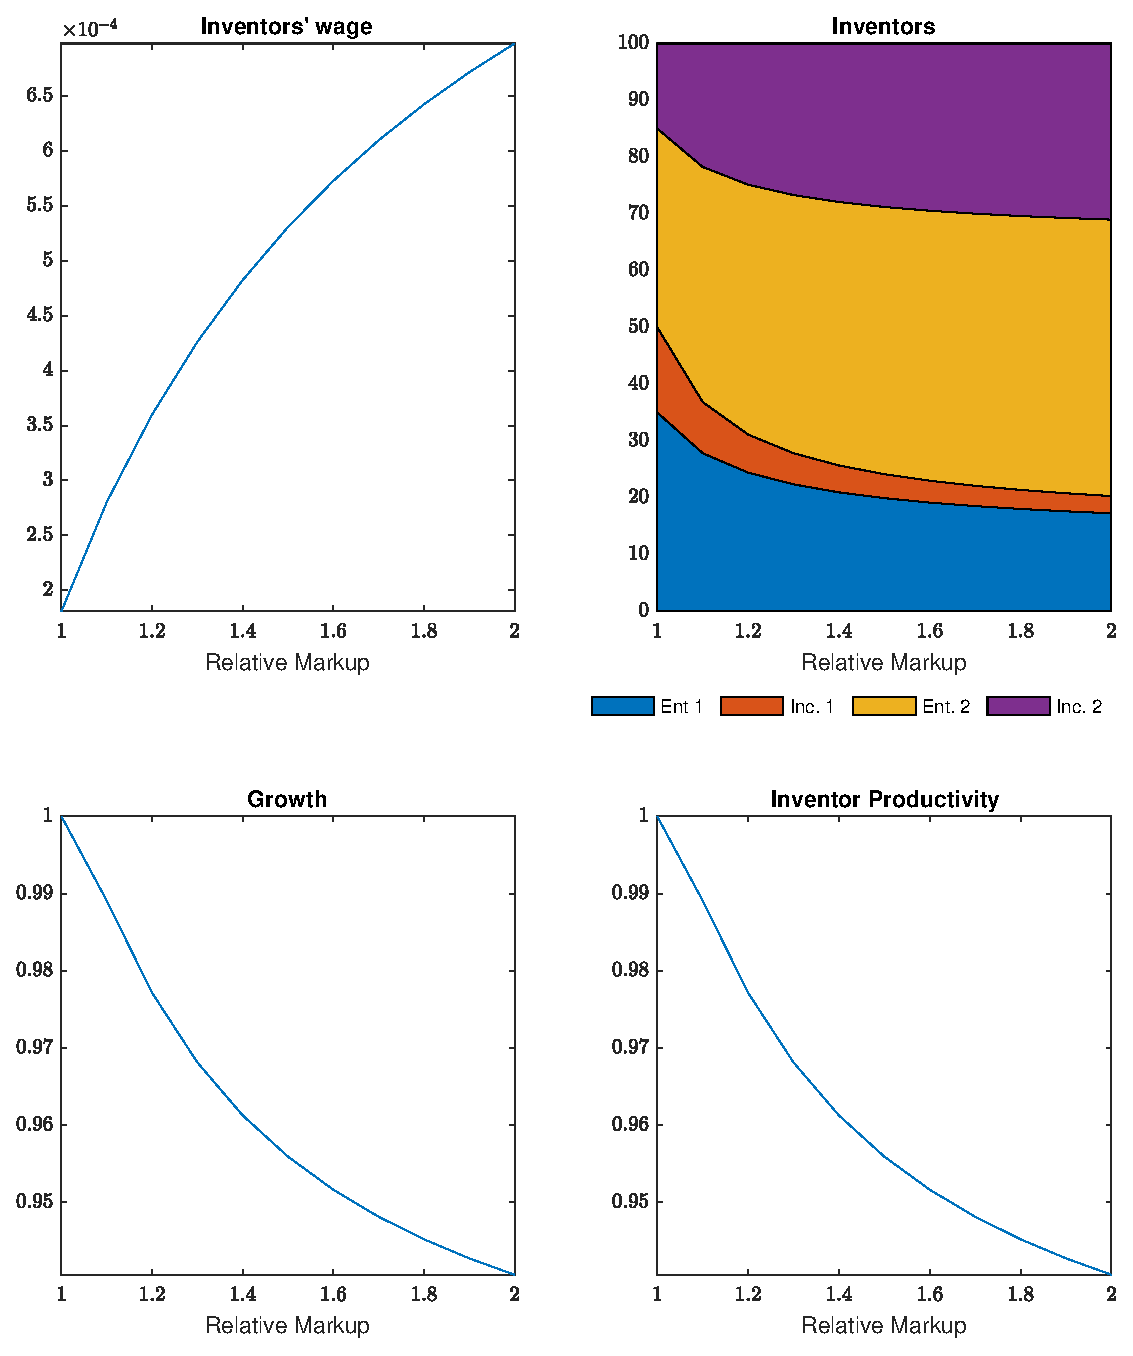
\includegraphics[width=1\columnwidth]{graphs/GE_aggregates}
\par\end{centering}
\raggedright{}{\small{}Note: This figure reports the comparative statics
for normalized profits, inventors, growth and inventor productivity
in the two-sector model. In all figures, the x-axis reports the markup
of sector 2 relative to sector 1. The parameters used to produce this
Figure are reported in Tables \ref{tab: extPar} and \ref{tab: intPar}.}{\small\par}
\end{figure}
\begin{figure}[th]
\begin{centering}
\caption{Comparative Statics in Sector 2's Markup Relative to Sector 1 in the
Two-Sector Model, Sector-level Aggregates \label{fig:TwoSecSectors}}
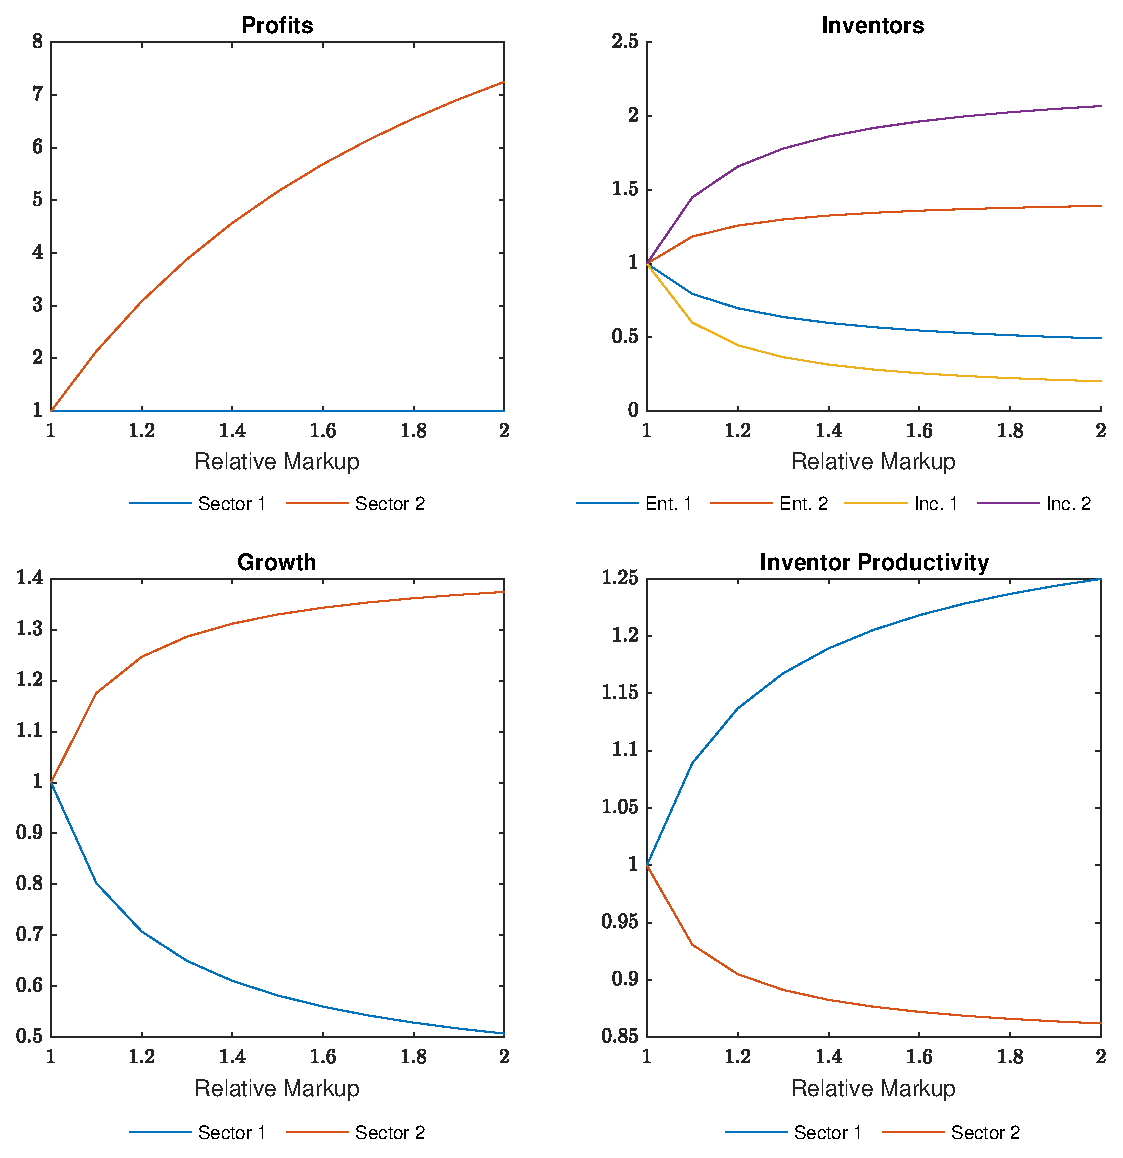
\includegraphics[width=1\textwidth]{graphs/GE_sectors}
\par\end{centering}
\raggedright{}{\small{}Note: This figure reports the comparative statics
for normalized profits, inventors, growth and inventor productivity
in the two-sector model. In all figures, the x-axis reports the markup
of sector 2 relative to sector 1. The parameters used to produce this
Figure are reported in Tables \ref{tab: extPar} and \ref{tab: intPar}.}{\small\par}
\end{figure}
\FloatBarrier

\subsubsection{Growth-Maximizing Policy}

I now turn to solve numerically for the combination of R\&D subsidies
that maximizes growth. I assume that the planner wishes to maximize
growth under a set of different constraint on the instruments available.
In particular, I assume that the planner cannot alter the nature of
innovation, that is, the planner cannot distinguish productive from
unproductive projects, and cannot forbid depositing patents that have
no productive value. In this model, eliminating protection for incumbents
would lead to a first-best where only entrants conduct R\&D, and reallocation
could only be beneficial to growth, as discussed in the previous section. 

I start from the 2012 equilibrium of my model economy, where the gap
in markups between sector 2 and sector 1 is 20\%, and all firms receive
a $19\%$ subsidy to inventors' wages and a 23\% tax on profits. I
then evaluate numerically three cost-neutral alternatives relative
to this benchmark, that is, I constrain the planner to leave the expenditure
on R\&D subsidies as a percentage of GDP fixed at the 2012 benchmark.
In the first scenario, the planner is allowed to distribute subsidies
freely, and can condition their reception on both the state of the
market (protected or unprotected) and the identity of the receiving
firm (entrant or incumbent). In the other two scenarios, I only allow
the planner to act on one of these dimensions at a time. That is,
the planner can either control the cross-sector distribution of funds,
but not the allocation across incumbents and entrants, or vice versa. 

The results of this exercise are presented in Table \ref{tab: Policy}.
The 2012 equilibrium is reported in Columns 1 and 2. For reference,
the 1997 calibrated model has two identical sectors, that share the
stock of inventors equally, and within each sector incumbents have
30.3\% of the overall inventors employed, and GDP growth is 3\% per
annum, as reported in Table \ref{tab: intPar}. In the 2012 baseline,
the distribution of inventors is tilted towards the second sector,
where markups have increased, which results in a fall in annual GDP
growth of .07pp, about 2.5\% of the 1997 benchmark. As shown in the
graphs above, this new equilibrium sees a larger share of inventors
allocated to incumbents in the second sectors, which increases its
growth relative to its more competitive counterpart, and sees a decline
in productivity resulting from higher defensive innovation. Column
3 and 4 report the optimal cost-neutral R\&D subsidies chosen by a
growth-maximizing planner. Somewhat surprisingly, the most efficient
allocation of funds turns out to be an entry subsidy to entrants in
the more concentrated sector only. However, this result can be easily
rationalized through the findings in Figure \ref{fig:TwoSecSectors}.
As discussed above, the outflow of inventors from sector 1 increases
inventor productivity due to reduced defensive innovation. It is therefore
more efficient to leave entry unchanged in sector 1, and act directly
on the inventors' misallocation occurring in sector 2. This intuition
is confirmed by the results for the scenario in which the planner
can only allocate R\&D subsidy to one of the sector, but cannot condition
on the identity of the firm. In this case, subsidies are in part used
to increase incumbents' defensive innovation, which is also made more
attractive by the overall increase in entry. While this policy does
allow the planner to recover most of the lost ground relative to the
1997 equilibrium, bringing growth up to 2.99\%, it is still not as
effective as alternative cost-equivalent policies. In particular,
an alternative that might be easily implementable is a blanket entry
subsidy as reported in Columns 6 and 7, which achieves a growth in
annual output of 3.38\%, which is above the starting 1997 equilibrium. 

To conclude, the policy analysis suggests that entry subsidies are
the most effective policy to contrast the friction introduced by defensive
innovation in this model economy. In particular, it is best to subsidize
entrants in less competitive sectors, where this friction is most
pronounced, which increases growth by 0.5pp per annum. A more feasible
uniform R\&D subsidy to entrants produces quantitatively similar effects.
Conversely, sector-specific subsidies to reallocate inventors to more
competitive sectors are less effective, since they get channeled to
incumbents who employ them to conduct pre-emptive innovation, precisely
the source of inefficiency that the planner wishes to contrast.

\begin{sidewaystable}

\caption{Comparison of R\&D Policies in the Two-Sector Model}
\label{tab: Policy}
\begin{centering}
\begin{tabular}{l  <{\onslide<1->}d<{\onslide<1->}d<{\onslide<2->} HH d<{\onslide<2->}d<{\onslide<4->}d<{\onslide<4->}d<{\onslide<5->}d<{\onslide<5->} d<{\onslide}}
& \multicolumn{2}{c}{Baseline} &	\multicolumn{2}{H}{Optimal Subsidies} & \multicolumn{2}{c}{Optimal Cost-Neutral} & \multicolumn{2}{c}{Cost-Neutral Sector}  & \multicolumn{2}{c}{Cost-Neutral Entry}  \\
\midrule
&Sector \ 1 & Sector \ 2 & Sector \ 1 & Sector \ 2 & Sector \ 1 & Sector \ 2 & Sector \ 1 & Sector \ 2 & Sector \ 1 &Sector \ 2 \\ 
&(1)&(2)&(3)&(4)&(3)&(4)&(5)&(6)&(7)&(8)\\ \midrule 
\textsl{R\&D Subsidies:} \\ 
%$\tau$ & $23\%$ & $23\%$ & $23\%$ & $23\%$ & $23\%$ & $23\%$ & $23\%$ & $23\%$ & $23\%$ & $23\%$ \\ 
$s_{I}$ &\marktopleft{b1} $19\%$ & $19\%$ & $0\%$ & $0\%$ & \marktopleft{b3}$0\%$ & $0\%$ &  \marktopleft{b8}$46.17\%$ & $0\%$ & $0\%$ & $0\%$  \\ 
$s_e$ & $19\%$ & $19\%$ \markbottomright{b1}{red} & $1\%$ & $75.39\%$ & $0\%$ & $41.78\%$ \markbottomright{b3}{red} & $46.17\%$ & $0\%$ \markbottomright{b8}{red}&\marktopleft{b12} $29\%$ & $29\%$   \markbottomright{b12}{red} \\ 
\\[-.2cm]
\textsl{Aggregates:}\\ 
$L^{RD}_{I}$ &\marktopleft{b10} $6.70$ & \marktopleft{b5} $24.87$ & $24.87$ & $4.47$ & $6.37$ & \marktopleft{b6} $15.95$ &\marktopleft{b7} $10.83$ & $19.51$ & $4.83$ & $18.45$ \\ 
$L^{RD}_{e}$ & $24.41$  \markbottomright{b10}{red} & $44.02$ \markbottomright{b5}{red} & $23.12$ & $66.57$ & $23.87$ & $53.81$\markbottomright{b6}{red}& $30.24$ \markbottomright{b7}{red}& $39.42$ & $27.41$ & $49.30$ \\ 
$L^{RD}_{TOT}$ &\marktopleft{b2} $31.11$ & $68.89$ & $28.96$ &  $71.04$ &\marktopleft{b4} $30.25$ & $69.75$ & $41.07$ & $58.93$ & $32.25$ & $67.75$ \\ 
Sector Growth &$2.12\%$ & $3.74\%$  & &  & $2.08\%$ & $4.78\%$ & $2.61\%$ & $3.36\%$ & $2.45\%$ & $4.31\%$ \\ 
\midrule
GDP Growth &  \multicolumn{2}{c}{\onslide<1->{\marktopleft{b11}$2.93\%$}}  \markbottomright{b2}{red}  & \multicolumn{2}{H}{$3.15\%$} & \multicolumn{2}{c}{\onslide<2-> \marktopleft{b14}$3.43\%$} \markbottomright{b4}{red}   & \multicolumn{2}{c}{\onslide<4-> \marktopleft{b9} $2.99\%$} \markbottomright{b9}{red}& \multicolumn{2}{c}{\onslide<5-> \marktopleft{b13} $3.38\%$} {\onslide<1->} \markbottomright{b13}{red} \\ \hline %
%Subsidy/GDP & $0.20\%$ & $0.36\%$ & $0\%$ & $1.66\%$ & $0\%$ & $0.56\%$ & $0.55\%$ & $0\%$ & $0.22\%$ & $0.34\%$ \\ 
%Revenue/GDP & $1.02\%$ & $2.32\%$ & $1.02\%$ & $2.32\%$ & $1.02\%$ & $2.32\%$ & $1.02\%$ & $2.32\%$ & $1.02\%$ & $2.32\%$ \\ 

\end{tabular}
\uncover<1-2>{\tikz[overlay,remember picture,inner sep=1pt] \node[draw=red,rounded corners,fit=(marker-b1-a.north west) (marker-b1-b.south east)] {};}
\uncover<1-2>{\tikz[overlay,remember picture,inner sep=1pt] \node[draw=red,rounded corners,fit=(marker-b2-a.north west) (marker-b2-b.south east)] {};}
\uncover<2>{\tikz[overlay,remember picture,inner sep=1pt] \node[draw=red,rounded corners,fit=(marker-b3-a.north west) (marker-b3-b.south east)] {};}
\uncover<2>{\tikz[overlay,remember picture,inner sep=1pt] \node[draw=red,rounded corners,fit=(marker-b4-a.north west) (marker-b4-b.south east)] {};}
\uncover<3>{\tikz[overlay,remember picture,inner sep=1pt] \node[draw=red,rounded corners,fit=(marker-b5-a.north west) (marker-b5-b.south east)] {};}
\uncover<3>{\tikz[overlay,remember picture,inner sep=1pt] \node[draw=red,rounded corners,fit=(marker-b6-a.north west) (marker-b6-b.south east)] {};}
\uncover<4>{\tikz[overlay,remember picture,inner sep=1pt] \node[draw=red,rounded corners,fit=(marker-b7-a.north west) (marker-b7-b.south east)] {};}
\uncover<4>{\tikz[overlay,remember picture,inner sep=1pt] \node[draw=red,rounded corners,fit=(marker-b8-a.north west) (marker-b8-b.south east)] {};}
\uncover<4>{\tikz[overlay,remember picture,inner sep=1pt] \node[draw=red,rounded corners,fit=(marker-b9-a.north west) (marker-b9-b.south east)] {};}
\uncover<4>{\tikz[overlay,remember picture,inner sep=1pt] \node[draw=red,rounded corners,fit=(marker-b10-a.north west) (marker-b10-b.south east)] {};}
\uncover<4>{\tikz[overlay,remember picture,inner sep=1pt] \node[draw=red,rounded corners,fit=(marker-b11-a.north west) (marker-b2-b.south east)] {};}

\uncover<5-6>{\tikz[overlay,remember picture,inner sep=1pt] \node[draw=red,rounded corners,fit=(marker-b12-a.north west) (marker-b12-b.south east)] {};}
\uncover<5-6>{\tikz[overlay,remember picture,inner sep=1pt] \node[draw=red,rounded corners,fit=(marker-b13-a.north west) (marker-b13-b.south east)] {};}
\uncover<6>{\tikz[overlay,remember picture,inner sep=1pt] \node[draw=red,rounded corners,fit=(marker-b14-a.north west) (marker-b4-b.south east)] {};}
\uncover<6>{\tikz[overlay,remember picture,inner sep=1pt] \node[draw=red,rounded corners,fit=(marker-b11-a.north west) (marker-b2-b.south east)] {};}\\
\par\end{centering}
\raggedright{}{\small{}Note: The figures reported in this Table give
the optimal allocation of R\&D subsidies and the resulting aggregate
outcomes for a planner wishing to maximize aggregate growth in the
economy. The column headings refer to the various scenarios described
above. ``Baseline'' refers to the subsidy allocation reflecting
the 2012 equilibrium, where subsidies do not condition on sectors
or the position of firms within sectors; ``Optimal Cost-Neutral''
refer to the scenario where the planner is allowed to freely allocate
R\&D subsidies subject to the constraint that overall R\&D subsidy
expenditure as a percentage of GDP is held fixed at its 2012 benchmark;
``Cost-Neutral Sector'' consider a scenario where the planner can
choose which sector to allocate funds to, but not which firms within
the sector should receive the subsidy; ``Cost-Neutral Entry'' computes
the optimal universal entry subsidy, under the assumption that the
planner cannot condition its reception on the sector firms operate
in. }{\small\par}
\end{sidewaystable}

